\section{Durchführung}
\label{sec:Durchführung}
Für den Versuch wird der in \autoref{fig:schaltung1} dargestellte Versuchsaufbau verwendet, wobei auf einen XY-Schreiber verzichtet wurde, da die zu messenden Werte an den
Messgeräten abgelesen werden konten.

\begin{figure}[H]
    \centering
    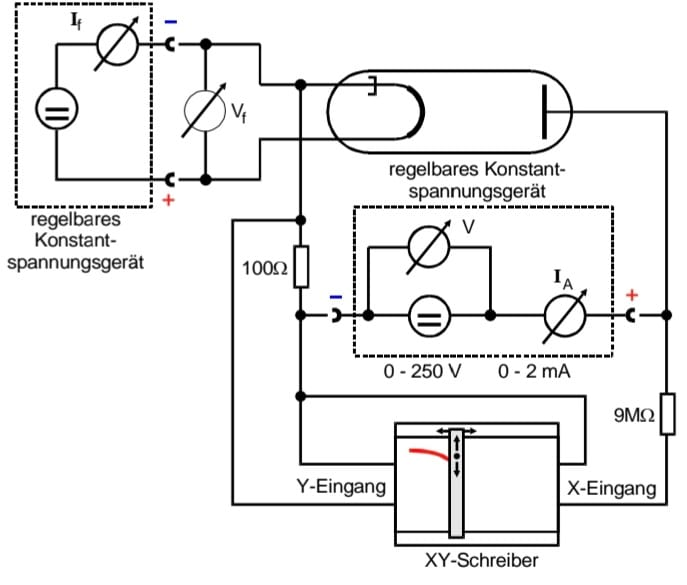
\includegraphics[width=0.5\textwidth]{data/schaltung1.jpeg}
    \caption{Schematische Darstellung des ersten Versuchsaufbaus\cite{Anleitung504}.}
    \label{fig:schaltung1}
\end{figure}

\noindent
Im ersten Teil des Versuches soll eine Kennlinienschar für die verwendete Hochvakuumdiode aufgenommen werden. Dabei wurden fünf verschiedene Stromstärken im
Bereich von 1,9 bis $\SI{2,5}{\ampere}$ für die Heizleistung verwendet. Für jede dieser fünf Messreihen wurde dann die Beschleunigungsspannung langsam erhöht und die
jeweiligen Werte für die Beschleunigungsspannung und den resultierenden Anodenstrom notiert. Dies wurde wiederholt, bis der Sättigungsstrom erreicht wurde, also sich
die Werte für den Anodenstrom garnicht mehr, oder nur noch sehr wenig verändert haben. Die Beschleunigungsspannung wurde dafür in Schritten von $\SI{4}{\volt}$ erhöht,
wobei am Spannungsgerät die anliegende Spannung ab $\SI{60}{\volt}$ nur noch in Schritten von $\SI{5}{\volt}$ ablesbar war. Desshalb wurden die Messintervalle nach
$\SI{60}{\volt}$ auf $\SI{5}{\volt}$ vergrößert.
\newline\newline
Im zweiten Teil des Versuches soll das Gebiet des Anlaufstromes untersucht werden. Dafür wird der Versuchsaufbau aus dem ersten Teil leicht abgewandelt. Der neue Aufbau
ist in \autoref{fig:schaltung2} abgebildet. 

\begin{figure}[H]
    \centering
    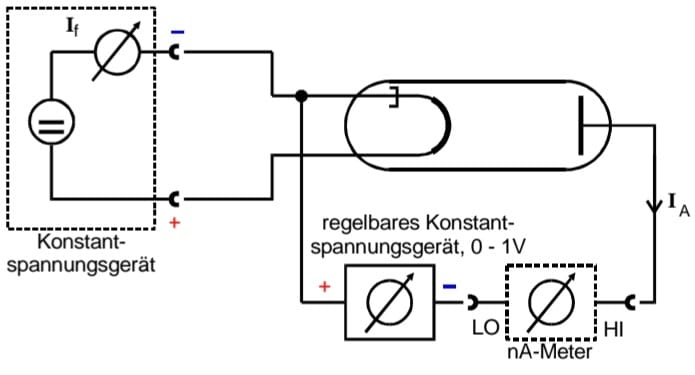
\includegraphics[width=0.5\textwidth]{data/schaltung2.jpeg}
    \caption{Schematische Darstellung des zweiten Versuchsaufbaus\cite{Anleitung504}.}
    \label{fig:schaltung2}
\end{figure}

\noindent
Es wird zunächst die maximal für die Anode zugelassene Heizleistung, mit einer Stromstärke von $\SI{2,5}{\ampere}$, eingestellt. Wie im ersten Teil des Versuches wird
anschleißend die Beschleunigungsspannung langsam erhöht, dies geschieht nun allerding in Schritten von $\SI{0,05}{\volt}$. Es werden erneut die jeweils resultierenden
Messwerte für den Anodenstrom mit den zugehörigen Werten der Beschleunigungsspannung notiert. Die maximale Beschleunigungsspannung war hierbei durch das verwendete
Spannungsgerät auf $\SI{0,95}{\volt}$ begrenzt.
